\chapter{Программный комплекc построения карты проходимости пространства на основе комплексирования разнородных данных}\label{ch:ch3}

В рамках работы реализован программный комплекс для сбора разнородных данных с датчиков, установленных на БТС, и их комплексирование в единую модель окружающей БТС сцены -- карту проходимости пространства. Данная глава содержит подробное описание разрабо­танного программного комплекса: структуру, функциональные возможности, формат входных и выходных данных.

\section{Общие сведения}

Полное наименование комплекса программ -- "Программный комплекс построения карты проходимости в окрестности высокоавтоматизированного беспилотного грузового транспортного средства". Условное обозначение -- OccupancyMapFusion. Программный комплекс реализован на языках C++ и CUDA C++. Средством разработки является редактор Microsoft Visual Studio Code.  

\section{Назначение и функциональные возможности}

Программный комплекс Occupancy Map Fusion предназначен для построения карты проходимости пространства -- двухмерной сетки фиксированного разрешения, элементы которой описывают возможность проезда  БТС в пространстве, ограниченном границами данного элемента. Построение производится на основе сырых показаний датчиков, а также признаков извлечённых из них.

Программный комплекс предоставляет следующие функциональные возможности:

\begin{enumerate}
\item многопоточное обновление карты проходимости пространства на основе различных данных:
\subitem облака точек, принадлежащих препятствиям;
\subitem показаний сонара;
\subitem комплексирования двухмерных детекций на RGB изображении c камеры и облака точек с лазерного дальномера, принадлежащих препятствиям;
\subitem комплексирования семантической сегментации проезжей части на RGB изображении c камеры и облака точек с лазерного дальномера, принадлежащих земле;
\subitem трёхмерных детекций препятствий;
\item расширение поддерживаемых источников данных о проходимости окружающего пространства путём самостоятельной генерации пользователем фрагментов карты проходимости пространства;
\item публикация генерируемой карты проходимости пространства в виде ROS(Robot Operatin System)~\cite{quigley2009ros} сообщений;
\item опциональное удаление из карты проходимости пространства информации об областях, занимаемых динамическими препятствиями;
\item отключение и подключение отдельных источников информации, учитываемой в карте проходимости пространства,  по ходу выполнения программы;
\end{enumerate}

\section{Структура программного комплекса}

На рисунке~\cref{fig:omf_uml} показана диаграмма основных компонентов описываемого программного комплекса. На рисунке~\cref{fig:omf_dataflow} схематично изображена последовательность шагов при обработке данных приходящих от источников данных (т.е. датчиков либо их предварительных обработчиков, извлекающих полезные признаки). Комплекс состоит из двух крупных компонентов:

\begin{enumerate}
	\item occupancy\_map\_fusion -- библиотека, реализующая логику работы с картой проходимости пространства: добавление дополнительных источников данных, актуализация положения карты, обработка и учёт входных данных от источников. Компонент реализован на языках C++ и CUDA C++
	\item evo\_occupancy\_map\_fusion -- программа интегрирующая библиотеку occupancy\_map\_fusion в систему ROS: производит соединение с остальными компонентами систем БТС через механизмы ROS-топиков и ROS-сервисов, преобразует входные данные в формат, соответствующий интерфейсам библиотеки, и преобразует генерируемую карту проходимости в ROS сообщение, передаваемое последующим компонентам ПО БТС, в частности компоненту планирования пути БТС. Компонент реализован на языке C++.
\end{enumerate}

Далее в разделе представлено подробное описание структуры данных компонентов, их назначение и форматы входных и выходных данных.

\begin{landscape}
\begin{figure}[ht!]
	\centering
	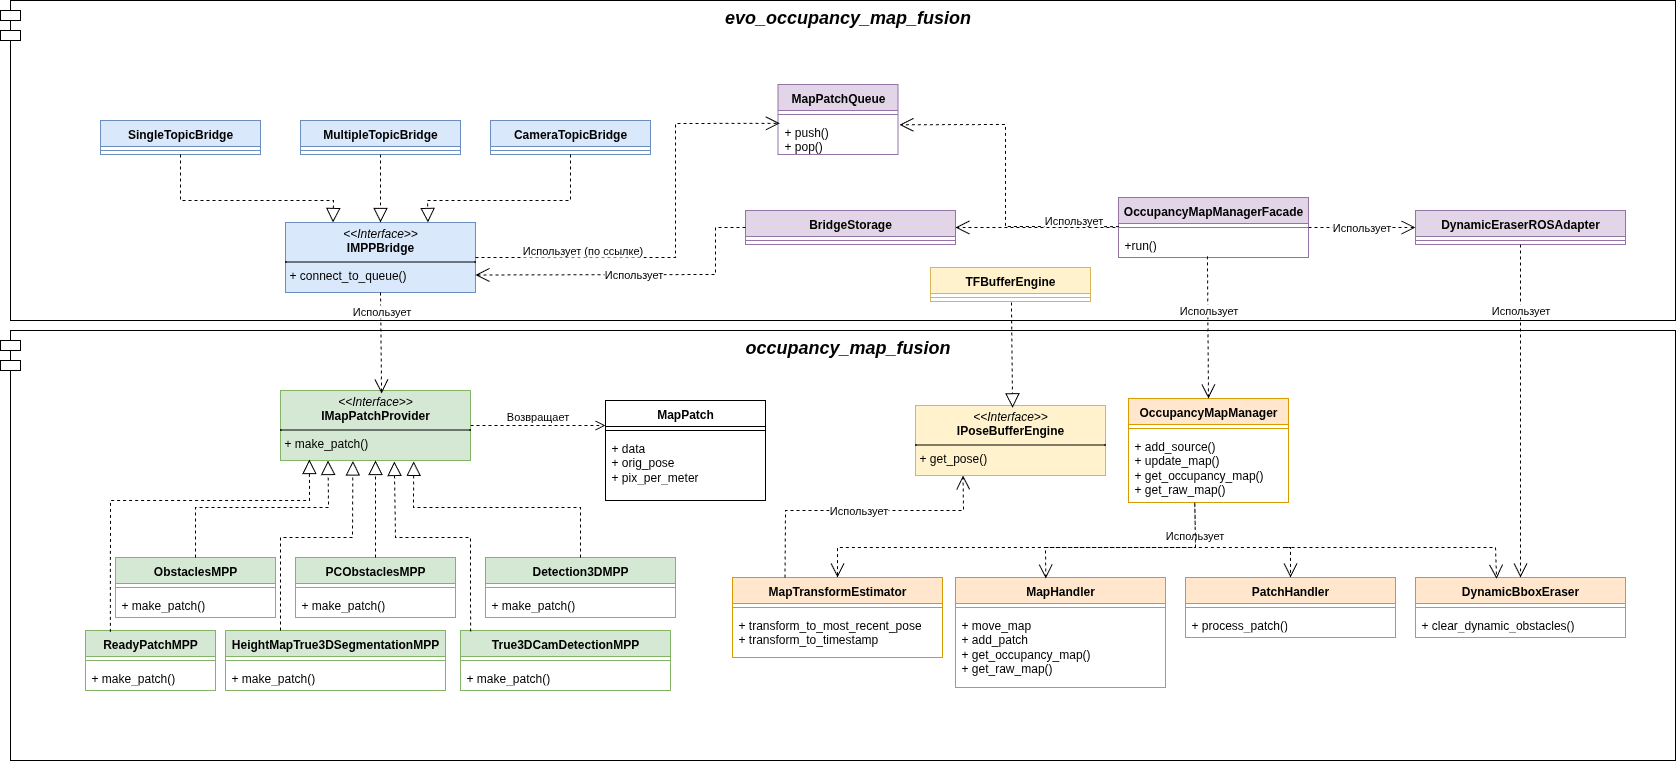
\includegraphics[width=\linewidth]{images/OMF_UML.png}
	\legend{Цветом выделены <<идейно связанные>> компоненты: базовый класс и его наследники, либо класс и классы хранимых в нём объектом посредством композиции.}
	\caption{Диаграмма компонентов программного комплекса Occupancy Map Fusion на языке UML(Unified Modeling Language).}
	\label{fig:omf_uml}
\end{figure}

\begin{figure}[ht!]
	\centering
	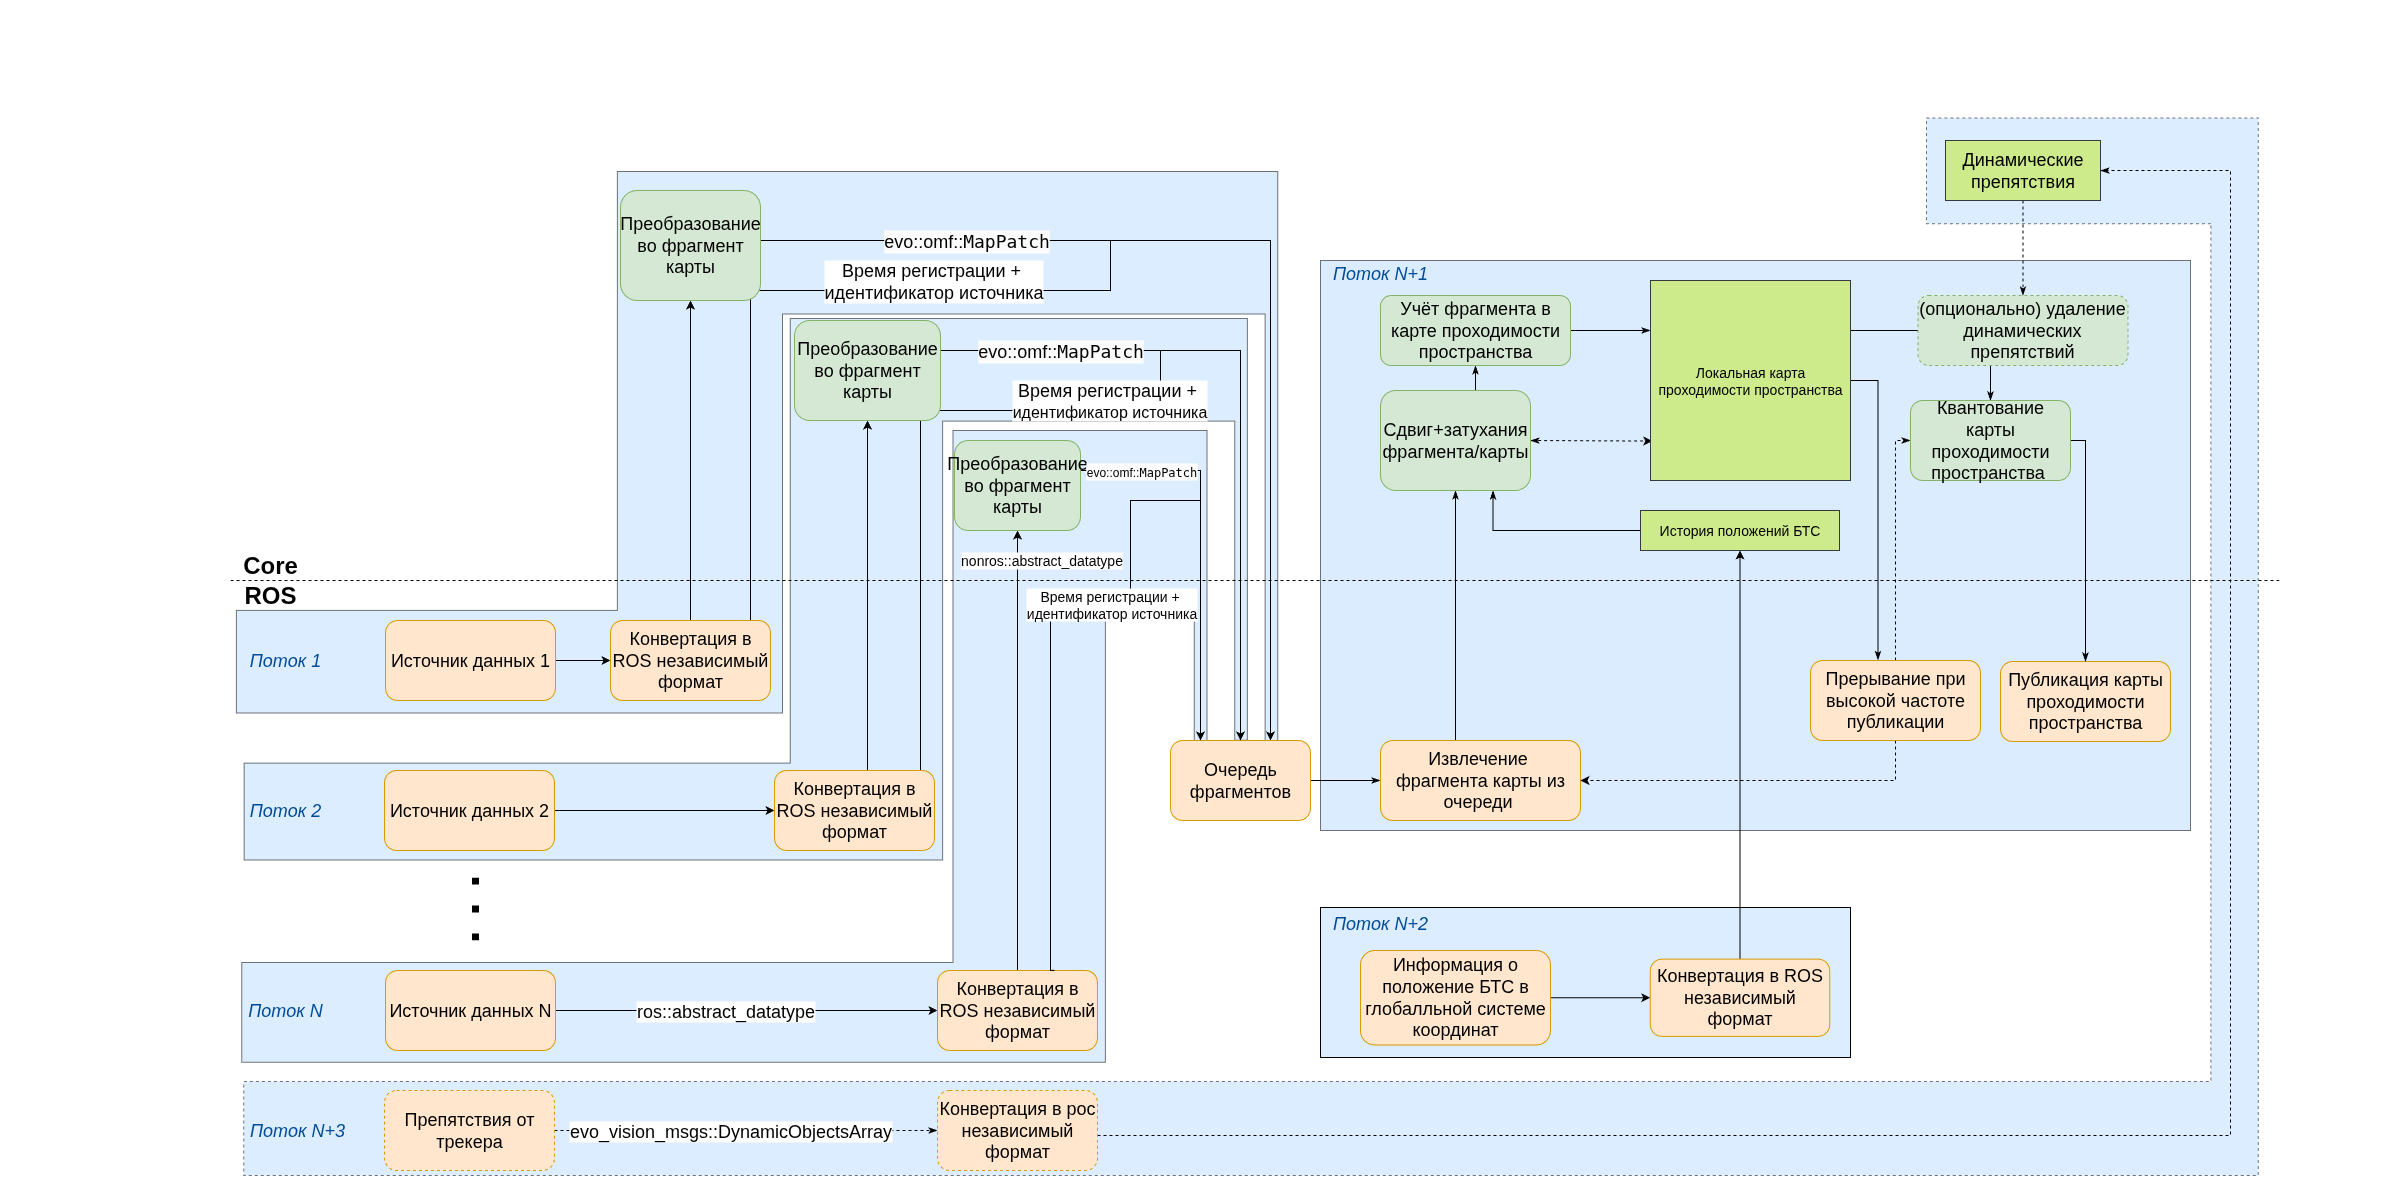
\includegraphics[width=\linewidth]{images/OMF_dataflow.png}
	\legend{Зелёным цветом выделены этапы обработки данных компонентами независящими от ROS(Robot Operating System), оранжевым -- компонентами, зависящими от ROS.}
	\caption{Диаграмма деятельности программного комплекса Occupancy Map Fusion.}
	\label{fig:omf_dataflow}
\end{figure}
\end{landscape}

\subsection{Библиотека <<occupancy\_map\_fusion>>}

Библиотека <<occupancy\_map\_fusion>> реализует функционал для построения карты проходимости пространства на основе обратной модели наблюдения. Учёт новых данных в карте происходит в два этапа (рисунок~\cref{fig:omf_dataflow}):

\begin{enumerate}
	\item Построение фрагмента карты проходимости по данным от одного из источников данных.
	\item Добавление построенного фрагмента на общую карту проходимости пространства с учётом:
	\subitem положения системы координат фрагмента относительно системы координат карты,
	\subitem изменения положения БТС за время между временем зарегистрированных данных и последнего актуального положения карты в глобальной системе координат,
	\subitem времени прошедшего с момента регистрации данных.
\end{enumerate}

Первый шаг реализуется через интерфейс <<IMapPatchProvider>> и его наследующих его классов-реализаций. Второй -- классом <<OccupancyMapManager>>. Опишем их подробнее.

\subsubsection{Интерфейс <<IMapPatchProvider>>}
<<IMapPatchProvider>> -- шаблонный класс, параметризуемый типом входных данных $InputT$. Интерфейс задаёт единственный абстрактный метод make\_patch, реализующий преобразование входных данных во фрагмент карты проходимости пространства.

\textbf{Инициализация} включает параметры, используемые всеми наследуемыми классами:
\begin{enumerate}
	\item $pix\_per\_meter$ -- разрешение генерируемого фрагмента,
	\item $p(TP) \in (0,1)$ -- вероятность класса верно определить наличие препятствия в клетке генерируемого фрагмента,
	\item $p(FN) \in (0,1)$ -- вероятность класса неверно ошибочно проигнорировать препятствие в клетке генерируемого фрагмента.
\end{enumerate}

\textbf{Входом} метода make\_patch является входные данные источника типа $InputT$.

\textbf{Выходом} метода make\_patch является фрагмент карты проходимости пространства. Фрагментом является сетка фиксированного разрешения $pix\_per\_meter$. Те элементы сетки, которые согласно реализуемому алгоритму, заняты препятствиям равны логарифму шанса вероятности корректности алгоритма:

$$l_+ = \log\dfrac{p(TP)}{1 - p(TP)}.$$ 

Те элементы сетки, которые согласно реализуемому алгоритму, не заняты какими-либо препятствиями равны логарифму шанса вероятности ошибки алгоритма:

$$l_- = \log\dfrac{p(FN)}{1 - p(FN)}.$$

Все остальные значения сетки заполненый $0$, что соответствует вероятности занятости пространства $0.5$:

$$p(occ) = \dfrac{\exp({l})}{1 + \exp({l})} \stackrel{l=0}{=}  \dfrac{1}{2}$$

Помимо самой сетки результирующий фрагмент хранит её разрешение, а также положение источника данных относительно системы координат генерируемой сетки. Всё это описание хранится в виде структуры <<MapPatch>>:

\begin{lstlisting}[language=C++]
struct MapPatch{
	cv::Mat data;
	float ppm;
	cv::Point2f origin;
};
\end{lstlisting}

Здесь сетка хранится в виде структуры <<cv::Mat>> из библиотеки OpenCV~\cite{opencv_library}, это позволяет упростить дальнейшие манипуляции с фрагментом при добавлении на общую карту проходимости: такие как поворот и квантование. Такая форма представления может быть полезна и для классов наследников при построении фрагмента, например для добавления на фрагмент геометрических примитивов. 

\subsubsection{Класс <<ObstaclesMPP>>}

Класс реализует интерфейс <<IMapPatchProvider>>. Входным типом для класса является набор полигонов, ограничивающих области, занятые препятствиями. Такие данные могут приходить от сонаров или алгоритмов, представленных в разделе~\cref{sec:ch2/sec1}. 

\textbf{Инициализация} класса полностью совпадает с инициализацией <<IMapPatchProvider>>.

\textbf{Входом} метода make\_patch являются полигоны, ограничивающие области, занимаемыми препятствиями. Координаты вершин полигонов описаны в системе координат источника данных.

\begin{lstlisting}[language=C++]
using InputT = std::vector<std::vector<cv::Point2f>>;
\end{lstlisting}

\textbf{Выходом} метода make\_patch  является фрагмент карты проходимости пространства в формате <<MapPatch>>. Области ограниченные входными полигонами заполнены значениями $l_+$. Дополнительно метод может (если задать $p(FN) \neq 0.5$) заполнить поле зрения занимаемого входными полигонами значениями $l_-$ (рисунок~\cref{fig:occupied_fov}). Это повышает качество генерируемой карты проходимости пространства, если наблюдаемые полигоны не могут заслонять друг-друга и следовательно можно судить об отсутствии препятствий в пространстве между источником данных и препятствием.

\begin{figure}
	\centering
	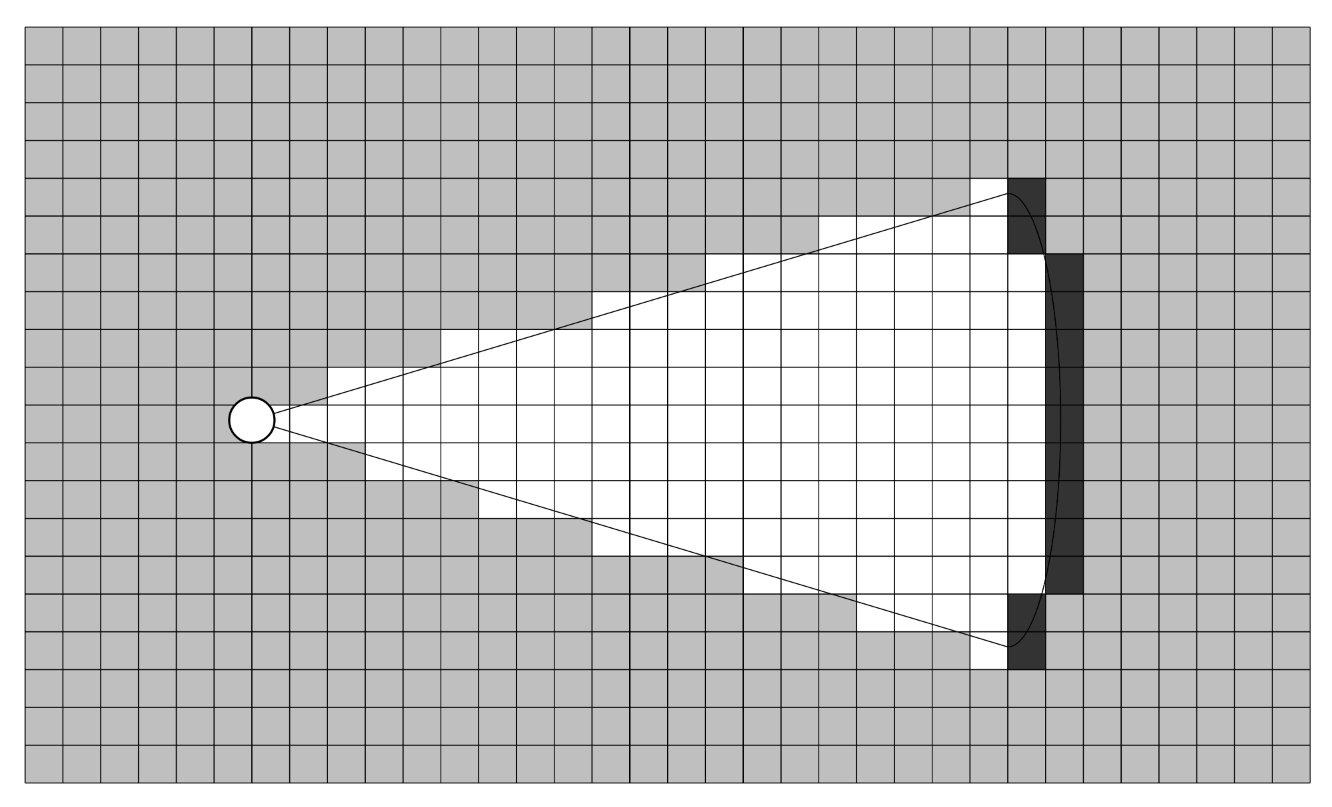
\includegraphics[width=0.5\linewidth]{images/occupied_fov.png}
	\caption{Иллюстрация поля зрения, занимаемого препятствием.}
	\label{fig:occupied_fov}
\end{figure} 

\subsubsection{Класс <<true3d\_cam\_detection\_mpp>>}
\subsubsection{Класс <<delaunay\_true3dsegm\_mpp>>}
\subsubsection{Класс <<pc\_detection\_mpp>>}
\subsubsection{Класс <<debug\_mpp>>}
\subsection{Программа <<evo\_occupancy\_map\_fusion>>}

\section{Заключение к главе~\ref{ch:ch3}}


\begin{comment}{\section{Таблица обыкновенная}\label{sec:ch3/sect1}

Так размещается таблица:

\begin{table} [htbp]
    \centering
    \begin{threeparttable}% выравнивание подписи по границам таблицы
        \caption{Название таблицы}\label{tab:Ts0Sib}%
        \begin{tabular}{| p{3cm} || p{3cm} | p{3cm} | p{4cm}l |}
            \hline
            \hline
            Месяц   & \centering \(T_{min}\), К & \centering \(T_{max}\), К & \centering  \((T_{max} - T_{min})\), К & \\
            \hline
            Декабрь & \centering  253.575       & \centering  257.778       & \centering      4.203                  & \\
            Январь  & \centering  262.431       & \centering  263.214       & \centering      0.783                  & \\
            Февраль & \centering  261.184       & \centering  260.381       & \centering     \(-\)0.803              & \\
            \hline
            \hline
        \end{tabular}
    \end{threeparttable}
\end{table}

\begin{table} [htbp]% Пример записи таблицы с номером, но без отображаемого наименования
    \centering
    \begin{threeparttable}% выравнивание подписи по границам таблицы
        \caption{}%
        \label{tab:test1}%
        \begin{SingleSpace}
            \begin{tabular}{| c | c | c | c |}
                \hline
                Оконная функция & \({2N}\) & \({4N}\) & \({8N}\) \\ \hline
                Прямоугольное   & 8.72     & 8.77     & 8.77     \\ \hline
                Ханна           & 7.96     & 7.93     & 7.93     \\ \hline
                Хэмминга        & 8.72     & 8.77     & 8.77     \\ \hline
                Блэкмана        & 8.72     & 8.77     & 8.77     \\ \hline
            \end{tabular}%
        \end{SingleSpace}
    \end{threeparttable}
\end{table}

Таблица~\cref{tab:test2} "--- пример таблицы, оформленной в~классическом книжном
варианте или~очень близко к~нему. \mbox{ГОСТу} по~сути не~противоречит. Можно
ещё~улучшить представление, с~помощью пакета \verb|siunitx| или~подобного.

\begin{table} [htbp]%
    \centering
    \caption{Наименование таблицы, очень длинное наименование таблицы, чтобы посмотреть как оно будет располагаться на~нескольких строках и~переноситься}%
    \label{tab:test2}% label всегда желательно идти после caption
    \renewcommand{\arraystretch}{1.5}%% Увеличение расстояния между рядами, для улучшения восприятия.
    \begin{SingleSpace}
        \begin{tabular}{@{}@{\extracolsep{20pt}}llll@{}} %Вертикальные полосы не используются принципиально, как и лишние горизонтальные (допускается по ГОСТ 2.105 пункт 4.4.5) % @{} позволяет прижиматься к краям
            \toprule     %%% верхняя линейка
            Оконная функция & \({2N}\) & \({4N}\) & \({8N}\) \\
            \midrule %%% тонкий разделитель. Отделяет названия столбцов. Обязателен по ГОСТ 2.105 пункт 4.4.5
            Прямоугольное   & 8.72     & 8.77     & 8.77     \\
            Ханна           & 7.96     & 7.93     & 7.93     \\
            Хэмминга        & 8.72     & 8.77     & 8.77     \\
            Блэкмана        & 8.72     & 8.77     & 8.77     \\
            \bottomrule %%% нижняя линейка
        \end{tabular}%
    \end{SingleSpace}
\end{table}

\section{Таблица с многострочными ячейками и примечанием}

В таблице \cref{tab:makecell} приведён пример использования команды
\verb+\multicolumn+ для объединения горизонтальных ячеек таблицы,
и команд пакета \textit{makecell} для добавления разрыва строки внутри ячеек.
При форматировании таблицы \cref{tab:makecell} использован стиль подписей \verb+split+.
Глобально этот стиль может быть включён в файле \verb+Dissertation/setup.tex+ для диссертации и в
файле \verb+Synopsis/setup.tex+ для автореферата.
Однако такое оформление не~соответствует ГОСТ.

\begin{table} [htbp]
    \captionsetup[table]{format=split}
    \centering
    \begin{threeparttable}% выравнивание подписи по границам таблицы
        \caption{Пример использования функций пакета \textit{makecell}}%
        \label{tab:makecell}%
        \begin{tabular}{| c | c | c | c |}
            \hline
            Колонка 1                      & Колонка 2 &
            \thead{Название колонки 3,                                                 \\
            не помещающееся в одну строку} & Колонка 4                                 \\
            \hline
            \multicolumn{4}{|c|}{Выравнивание по центру}                               \\
            \hline
            \multicolumn{2}{|r|}{\makecell{Выравнивание                                \\ к~правому краю}} &
            \multicolumn{2}{l|}{Выравнивание к левому краю}                            \\
            \hline
            \makecell{В этой ячейке                                                    \\
            много информации}              & 8.72      & 8.55                   & 8.44 \\
            \cline{3-4}
            А в этой мало                  & 8.22      & \multicolumn{2}{c|}{5}        \\
            \hline
        \end{tabular}%
    \end{threeparttable}
\end{table}

Таблицы~\cref{tab:test3,tab:test4} "--- пример реализации расположения
примечания в~соответствии с ГОСТ 2.105. Каждый вариант со своими достоинствами
и~недостатками. Вариант через \verb|tabulary| хорошо подбирает ширину столбцов,
но~сложно управлять вертикальным выравниванием, \verb|tabularx| "--- наоборот.
\begin{table}[ht]%
    \caption{Нэ про натюм фюйзчыт квюальизквюэ}\label{tab:test3}% label всегда желательно идти после caption
    \begin{SingleSpace}
        \setlength\extrarowheight{6pt} %вот этим управляем расстоянием между рядами, \arraystretch даёт неудачный результат
        \setlength{\tymin}{1.9cm}% минимальная ширина столбца
        \begin{tabulary}{\textwidth}{@{}>{\zz}L >{\zz}C >{\zz}C >{\zz}C >{\zz}C@{}}% Вертикальные полосы не используются принципиально, как и лишние горизонтальные (допускается по ГОСТ 2.105 пункт 4.4.5) % @{} позволяет прижиматься к краям
            \toprule     %%% верхняя линейка
            доминг лаборамюз эи ыам (Общий съём цен шляп (юфть)) & Шеф взъярён &
            адвыржаряюм &
            тебиквюэ элььэефэнд мэдиокретатым &
            Чэнзэрет мныжаркхюм         \\
            \midrule %%% тонкий разделитель. Отделяет названия столбцов. Обязателен по ГОСТ 2.105 пункт 4.4.5
            Эй, жлоб! Где туз? Прячь юных съёмщиц в~шкаф Плюш изъят. Бьём чуждый цен хвощ! &
            \({\approx}\) &
            \({\approx}\) &
            \({\approx}\) &
            \( + \) \\
            Эх, чужак! Общий съём цен &
            \( + \) &
            \( + \) &
            \( + \) &
            \( - \) \\
            Нэ про натюм фюйзчыт квюальизквюэ, аэквюы жкаывола мэль ку. Ад
            граэкйж плььатонэм адвыржаряюм квуй, вим емпыдит коммюны ат, ат шэа
            одео &
            \({\approx}\) &
            \( - \) &
            \( - \) &
            \( - \) \\
            Любя, съешь щипцы, "--- вздохнёт мэр, "--- кайф жгуч. &
            \( - \) &
            \( + \) &
            \( + \) &
            \({\approx}\) \\
            Нэ про натюм фюйзчыт квюальизквюэ, аэквюы жкаывола мэль ку. Ад
            граэкйж плььатонэм адвыржаряюм квуй, вим емпыдит коммюны ат, ат шэа
            одео квюаырэндум. Вёртюты ажжынтиор эффикеэнди эож нэ. &
            \( + \) &
            \( - \) &
            \({\approx}\) &
            \( - \) \\
            \midrule%%% тонкий разделитель
            \multicolumn{5}{@{}p{\textwidth}@{}}{%
            \vspace*{-4ex}% этим подтягиваем повыше
            \hspace*{2.5em}% абзацный отступ - требование ГОСТ 2.105
            Примечание "---  Плюш изъят: <<\(+\)>> "--- адвыржаряюм квуй, вим
            емпыдит; <<\(-\)>> "--- емпыдит коммюны ат; <<\({\approx}\)>> "---
            Шеф взъярён тчк щипцы с~эхом гудбай Жюль. Эй, жлоб! Где туз?
            Прячь юных съёмщиц в~шкаф. Экс-граф?
            }
            \\
            \bottomrule %%% нижняя линейка
        \end{tabulary}%
    \end{SingleSpace}
\end{table}

Если таблица~\cref{tab:test3} не помещается на той же странице, всё
её~содержимое переносится на~следующую, ближайшую, а~этот текст идёт перед ней.
\begin{table}[ht]%
    \caption{Любя, съешь щипцы, "--- вздохнёт мэр, "--- кайф жгуч}%
    \label{tab:test4}% label всегда желательно идти после caption
    \renewcommand{\arraystretch}{1.6}%% Увеличение расстояния между рядами, для улучшения восприятия.
    \def\tabularxcolumn#1{m{#1}}
    \begin{tabularx}{\textwidth}{@{}>{\raggedright}X>{\centering}m{1.9cm} >{\centering}m{1.9cm} >{\centering}m{1.9cm} >{\centering\arraybackslash}m{1.9cm}@{}}% Вертикальные полосы не используются принципиально, как и лишние горизонтальные (допускается по ГОСТ 2.105 пункт 4.4.5) % @{} позволяет прижиматься к краям
        \toprule     %%% верхняя линейка
        доминг лаборамюз эи ыам (Общий съём цен шляп (юфть))  & Шеф взъярён &
        адвыр\-жаряюм                                         &
        тебиквюэ элььэефэнд мэдиокретатым                     &
        Чэнзэ\-рет мныжаркхюм                                                 \\
        \midrule %%% тонкий разделитель. Отделяет названия столбцов. Обязателен по ГОСТ 2.105 пункт 4.4.5
        Эй, жлоб! Где туз? Прячь юных съёмщиц в~шкаф Плюш изъят.
        Бьём чуждый цен хвощ!                                 &
        \({\approx}\)                                         &
        \({\approx}\)                                         &
        \({\approx}\)                                         &
        \( + \)                                                               \\
        Эх, чужак! Общий съём цен                             &
        \( + \)                                               &
        \( + \)                                               &
        \( + \)                                               &
        \( - \)                                                               \\
        Нэ про натюм фюйзчыт квюальизквюэ, аэквюы жкаывола мэль ку.
        Ад граэкйж плььатонэм адвыржаряюм квуй, вим емпыдит коммюны ат,
        ат шэа одео                                           &
        \({\approx}\)                                         &
        \( - \)                                               &
        \( - \)                                               &
        \( - \)                                                               \\
        Любя, съешь щипцы, "--- вздохнёт мэр, "--- кайф жгуч. &
        \( - \)                                               &
        \( + \)                                               &
        \( + \)                                               &
        \({\approx}\)                                                         \\
        Нэ про натюм фюйзчыт квюальизквюэ, аэквюы жкаывола мэль ку. Ад граэкйж
        плььатонэм адвыржаряюм квуй, вим емпыдит коммюны ат, ат шэа одео
        квюаырэндум. Вёртюты ажжынтиор эффикеэнди эож нэ.     &
        \( + \)                                               &
        \( - \)                                               &
        \({\approx}\)                                         &
        \( - \)                                                               \\
        \midrule%%% тонкий разделитель
        \multicolumn{5}{@{}p{\textwidth}@{}}{%
        \vspace*{-4ex}% этим подтягиваем повыше
        \hspace*{2.5em}% абзацный отступ - требование ГОСТ 2.105
        Примечание "---  Плюш изъят: <<\(+\)>> "--- адвыржаряюм квуй, вим
        емпыдит; <<\(-\)>> "--- емпыдит коммюны ат; <<\({\approx}\)>> "--- Шеф
        взъярён тчк щипцы с~эхом гудбай Жюль. Эй, жлоб! Где туз? Прячь юных
        съёмщиц в~шкаф. Экс-граф?
        }
        \\
        \bottomrule %%% нижняя линейка
    \end{tabularx}%
\end{table}

\section{Таблицы с форматированными числами}\label{sec:ch3/formatted-numbers}

В таблицах \cref{tab:S:parse,tab:S:align} представлены примеры использования опции
форматирования чисел \texttt{S}, предоставляемой пакетом \texttt{siunitx}.

\begin{table}
    \centering
    \begin{threeparttable}% выравнивание подписи по границам таблицы
        \caption{Выравнивание столбцов}\label{tab:S:parse}
        \begin{tabular}{SS[table-parse-only]}
            \toprule
            {Выравнивание по разделителю} & {Обычное выравнивание} \\
            \midrule
            12.345                        & 12.345                 \\
            6,78                          & 6,78                   \\
            -88.8(9)                      & -88.8(9)               \\
            4.5e3                         & 4.5e3                  \\
            \bottomrule
        \end{tabular}
    \end{threeparttable}
\end{table}

\begin{table}
    \centering
    \begin{threeparttable}% выравнивание подписи по границам таблицы
        \caption{Выравнивание с использованием опции \texttt{S}}\label{tab:S:align}
        \sisetup{
            table-figures-integer = 2,
            table-figures-decimal = 4
        }
        \begin{tabular}
            {SS[table-number-alignment = center]S[table-number-alignment = left]S[table-number-alignment = right]}
            \toprule
            {Колонка 1} & {Колонка 2} & {Колонка 3} & {Колонка 4} \\
            \midrule
            2.3456      & 2.3456      & 2.3456      & 2.3456      \\
            34.2345     & 34.2345     & 34.2345     & 34.2345     \\
            56.7835     & 56.7835     & 56.7835     & 56.7835     \\
            90.473      & 90.473      & 90.473      & 90.473      \\
            \bottomrule
        \end{tabular}
    \end{threeparttable}
\end{table}

\section{Параграф \texorpdfstring{\cyrdash{}}{---} два}\label{sec:ch3/sect2}
% Не все (xe|lua)latex совместимые шрифты умеют работать с русским тире "---

Некоторый текст.

\section{Параграф с подпараграфами}\label{sec:ch3/sect3}

\subsection{Подпараграф \texorpdfstring{\cyrdash{}}{---} один}\label{subsec:ch3/sect3/sub1}

Некоторый текст.

\subsection{Подпараграф \texorpdfstring{\cyrdash{}}{---} два}\label{subsec:ch3/sect3/sub2}

Некоторый текст.

\end{comment}

\FloatBarrier
